
\title{Lab Report 08 - Shape Context}
\author{
        Manuel Galliker  14-921-969 \\
                manuelga@student.ethz.ch
}
\date{\today}

\documentclass[12pt]{article}
\usepackage{graphicx}
\usepackage{float}
\begin{document}
\maketitle


\section{1.  Shape Context Descriptors  }

The function sc compute() was implemented as described in the “Shape Matching and Object Recognition Using Shape Contexts” paper. By iteration over all the possible point combinations a polar histogram can be computed. This can then be used to calculate thetha and the radius. The range of the radius denoted by smallest r and biggest r. Are normalized.

\section{ Cost Matrix }

The cost matrix was computed according to the given formulaby iterating over all points and descriptors the cost can be found by summing up. 

\section{Hungarian Algorithm }

For the hungarian algorithm there was just a minor adjustment needed. It needs a square cost matrix and therefore it was decided to sample ramdom points using randperm at the beginning of the file shape matching.m.

\section{Thin Plate Splines }
Also this algorithm was implemented according to the assignement. With the given formulas and the function dist2 K, P and V could be obtained. With theese a linear system of equations can be contructed to obtain $\omega$ and a.

\section{Results }
Here the results of using the first and second heart images at the sixt iteration can be seen:

\vspace{5mm}
\begin{figure}[H]
	\centering
	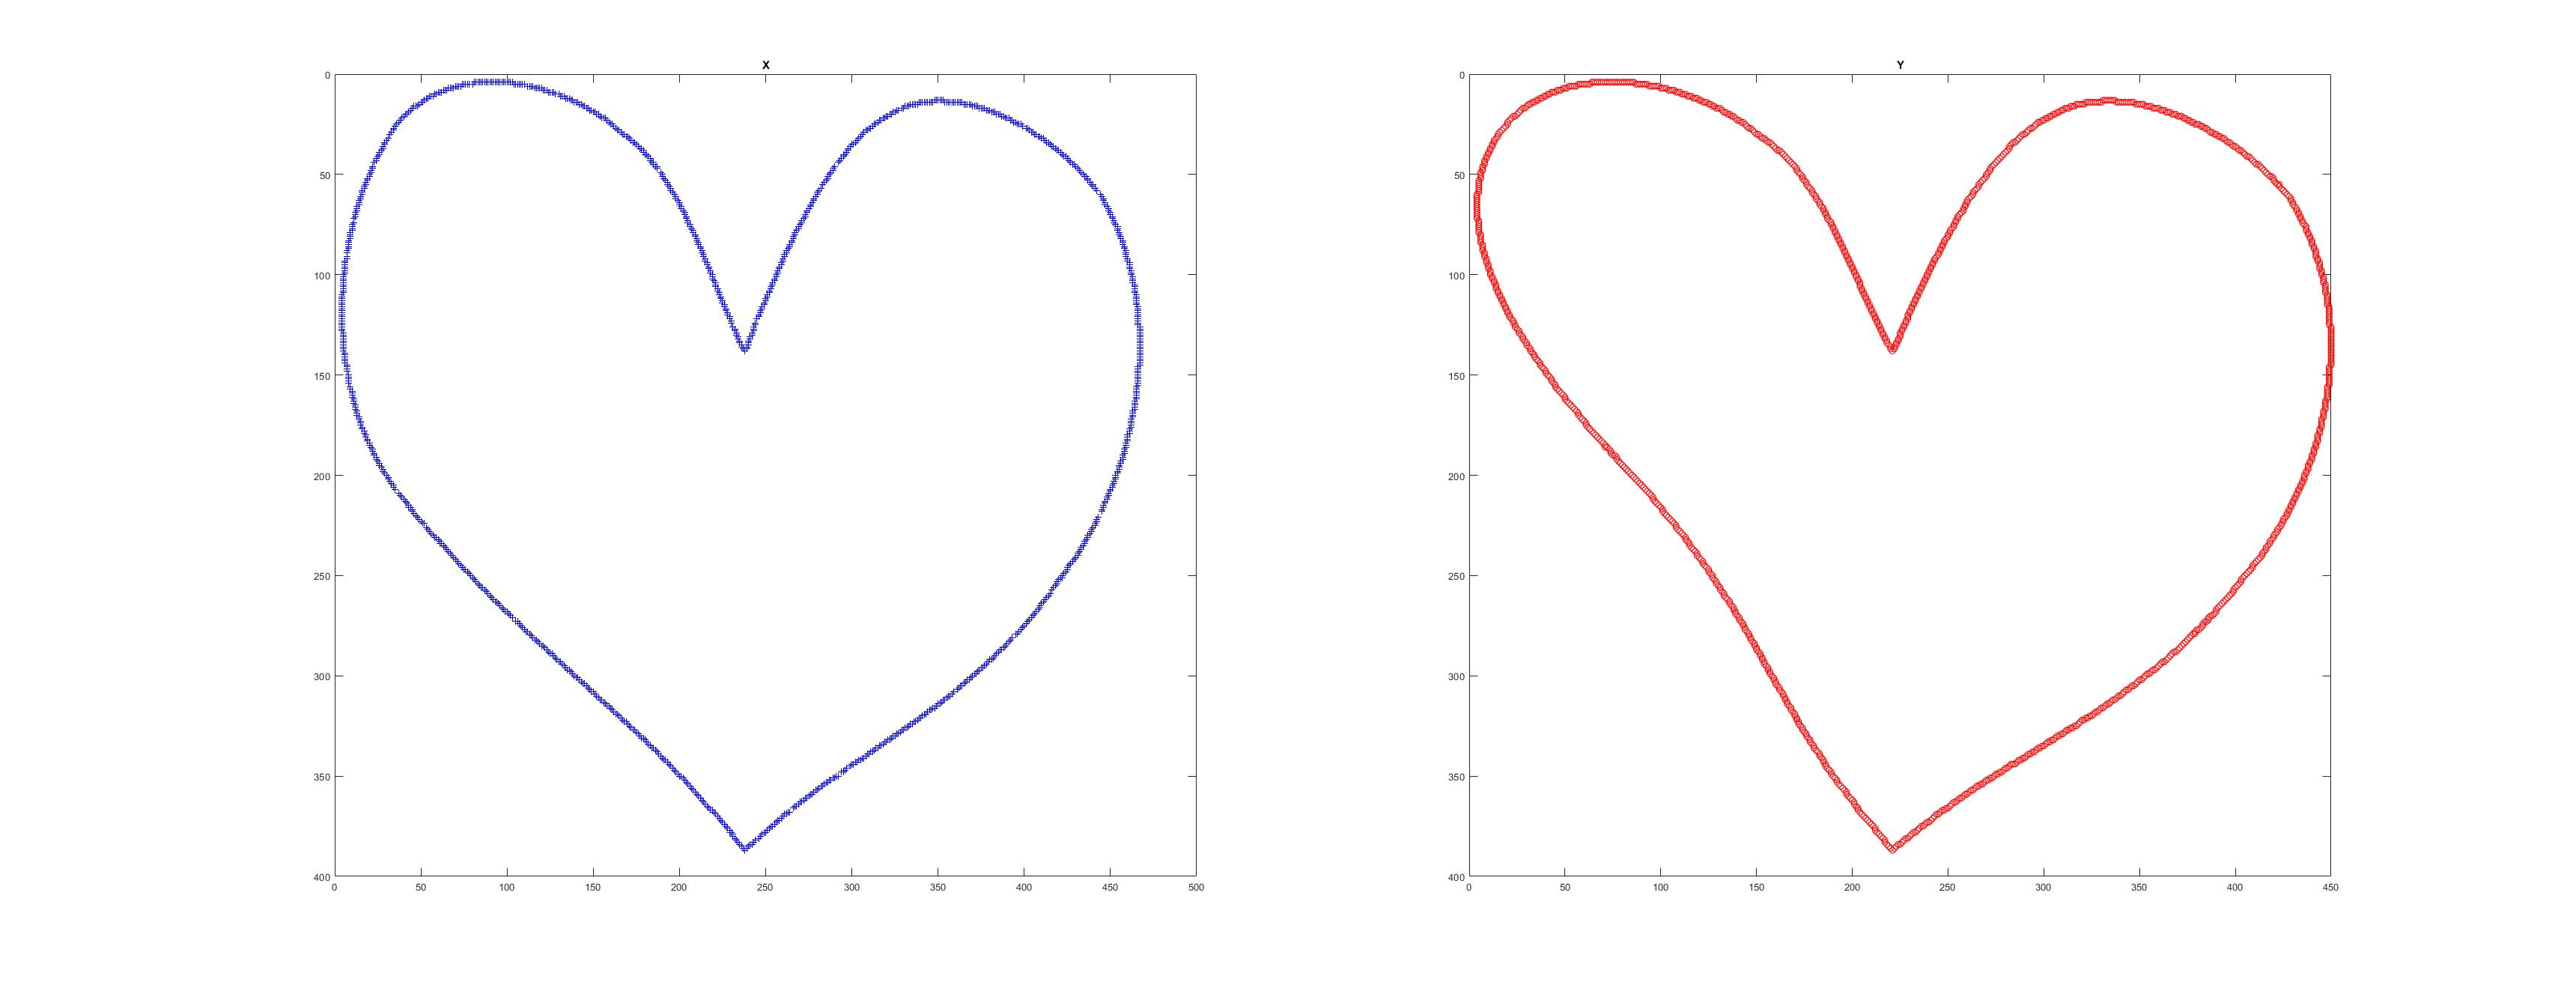
\includegraphics[width=1.1\textwidth]{1.jpg}
	\label{fig1}
\end{figure}
\vspace{5mm}
\vspace{5mm}
\begin{figure}[H]
	\centering
	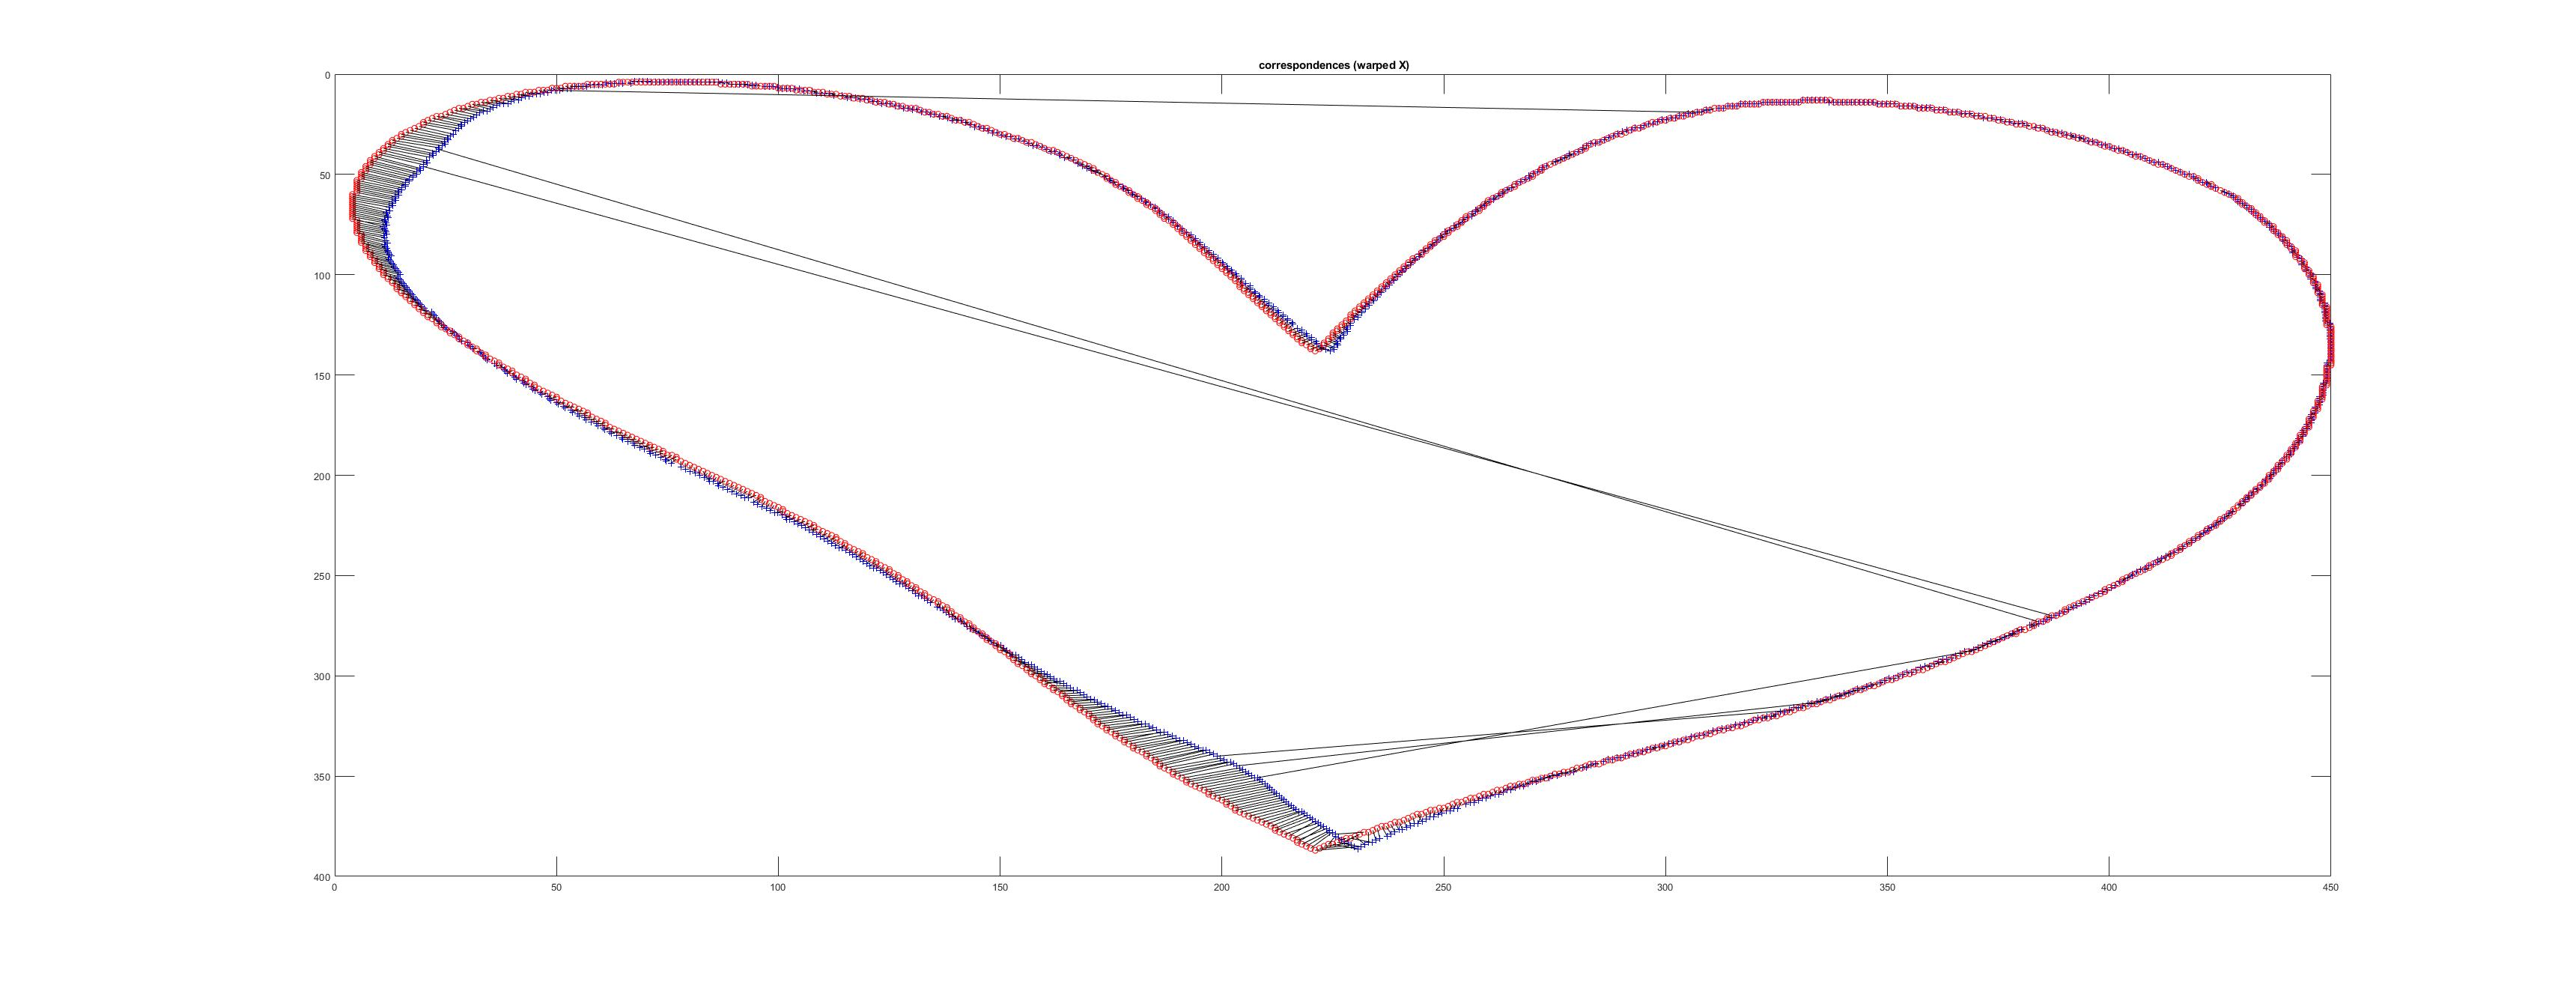
\includegraphics[width=1.1\textwidth]{2.jpg}
	\label{fig1}
\end{figure}
\vspace{5mm}

\vspace{5mm}
\begin{figure}[H]
	\centering
	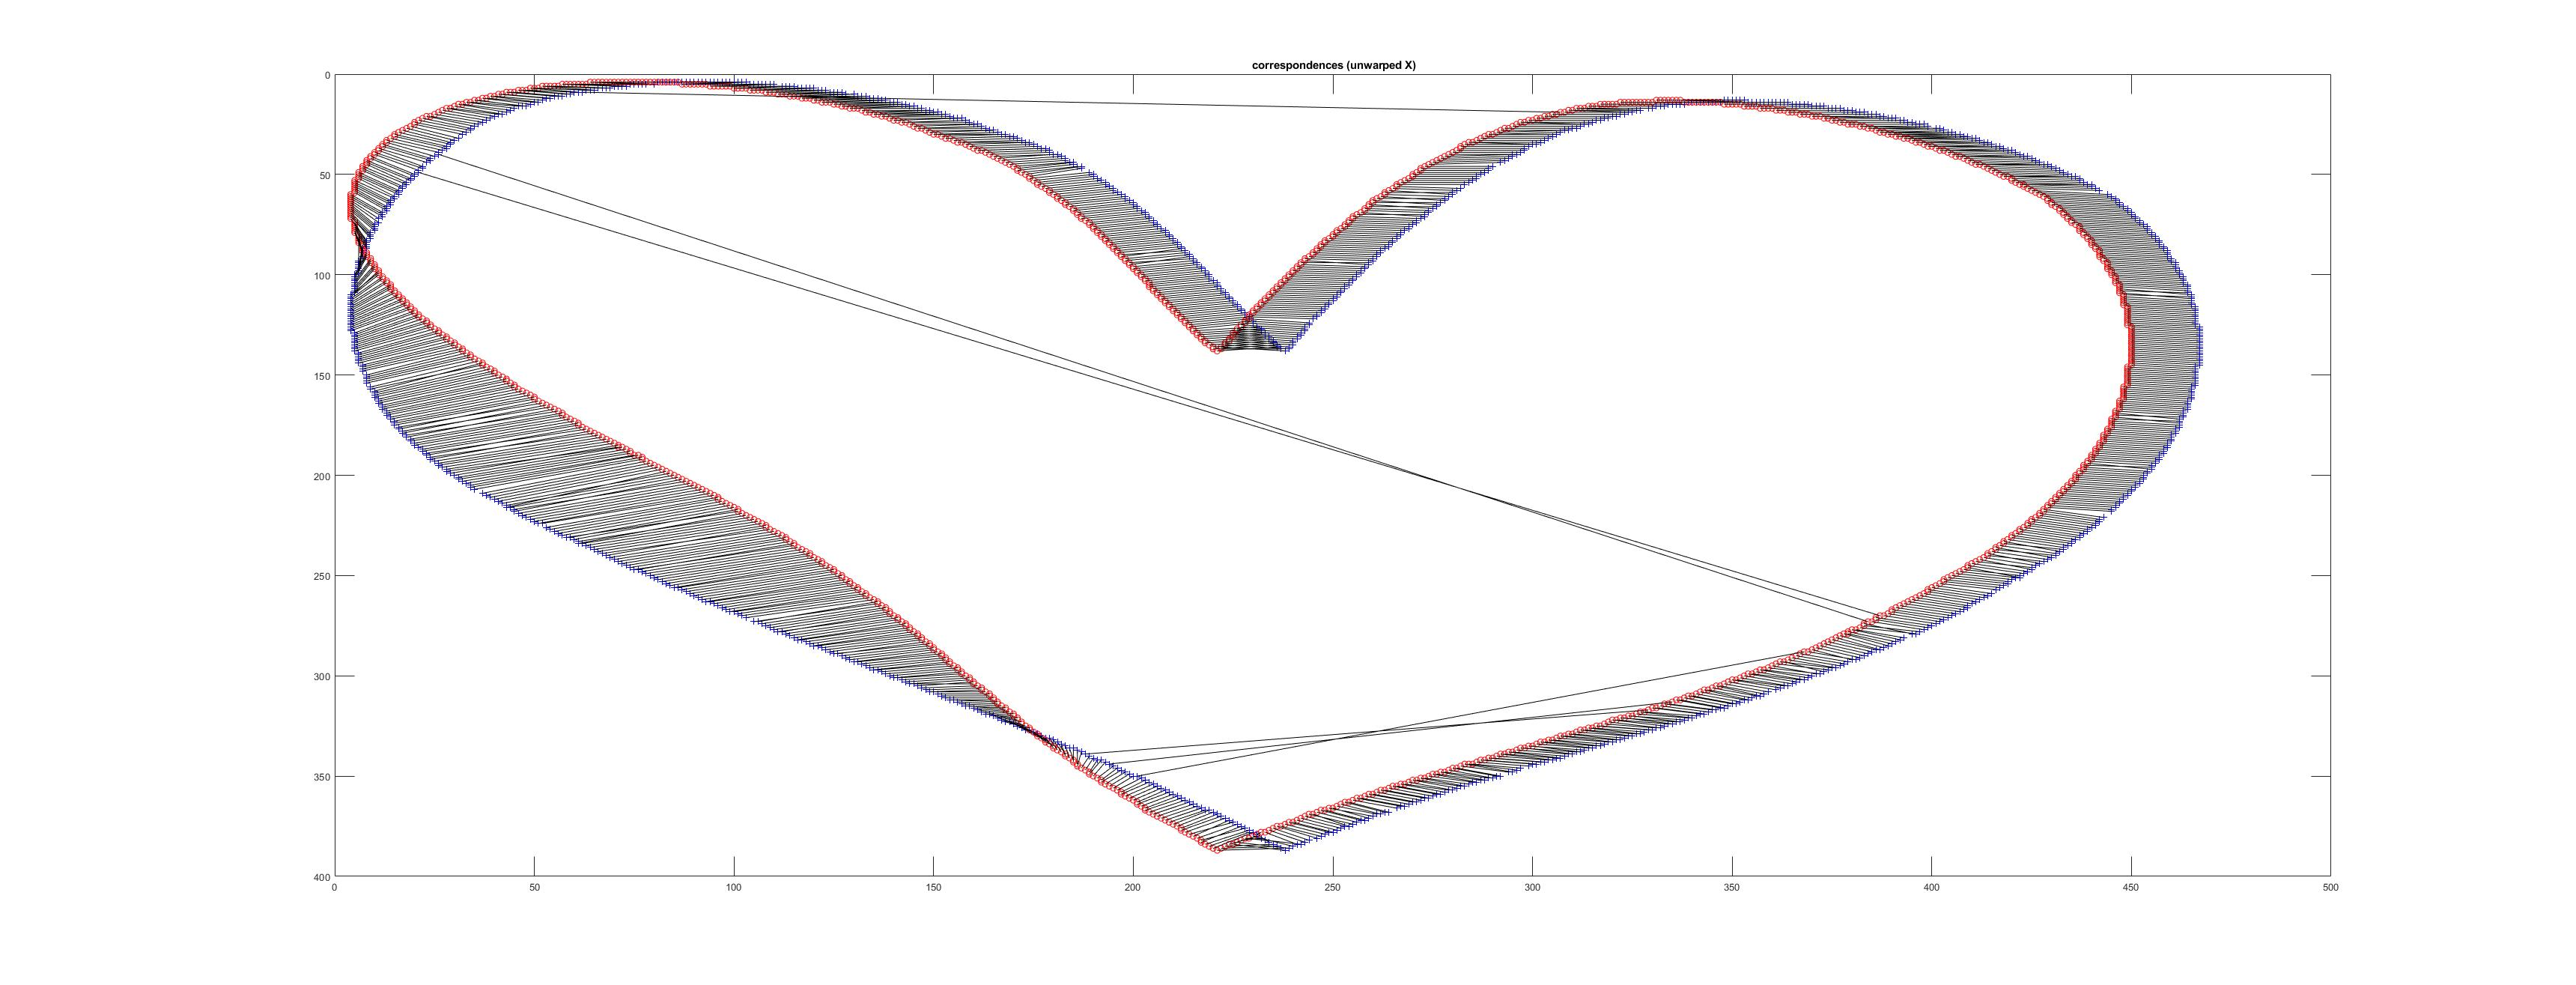
\includegraphics[width=1.1\textwidth]{3.jpg}
	\label{fig1}
\end{figure}
\vspace{5mm}

\vspace{5mm}
\begin{figure}[H]
	\centering
	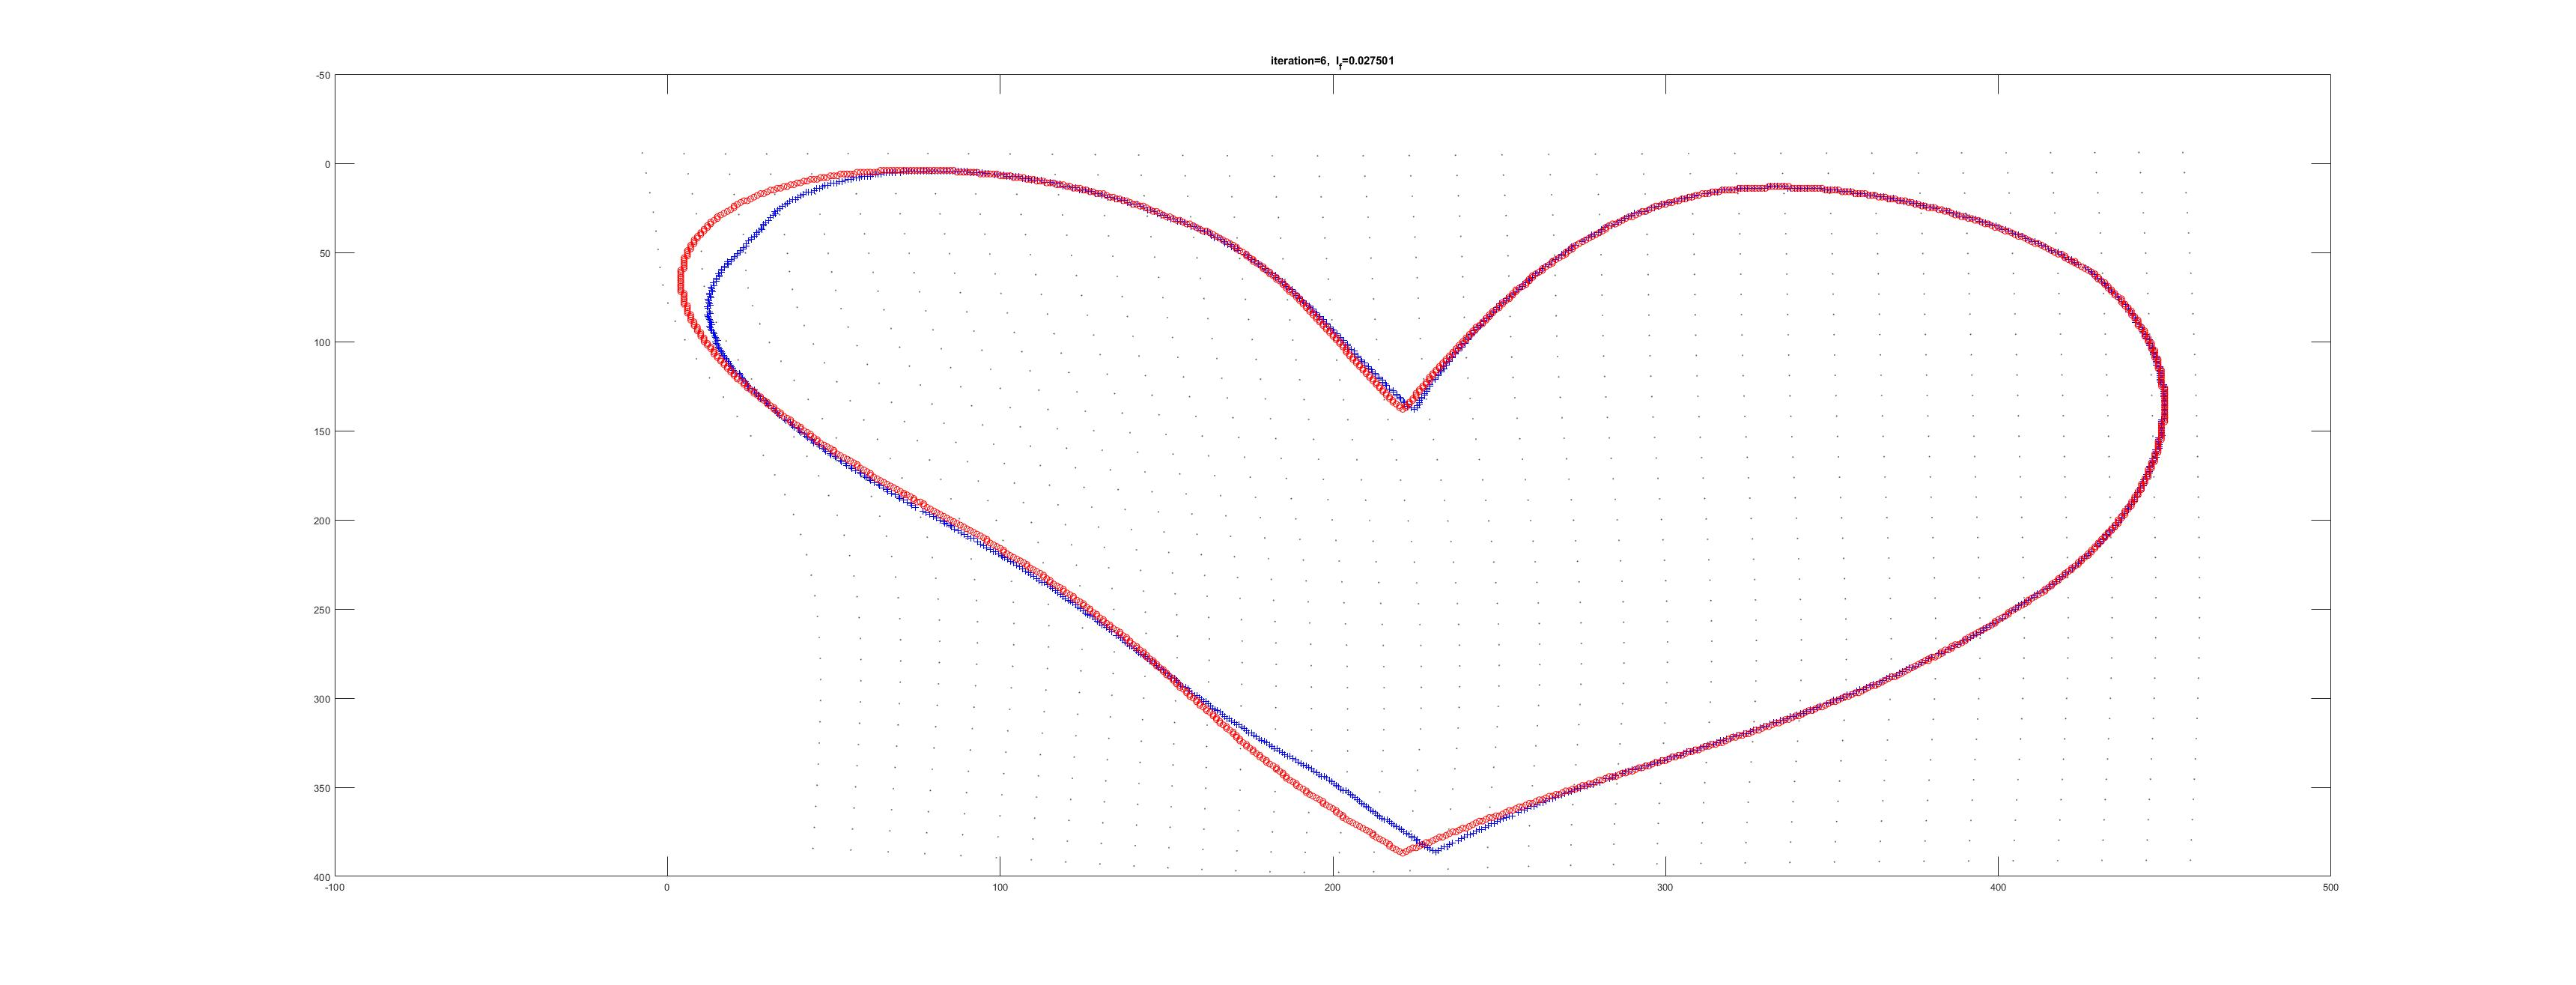
\includegraphics[width=1.1\textwidth]{4.jpg}
	\label{fig1}
\end{figure}
\vspace{5mm}

\section{Conclusion and Discussion}

As can be seen there are a couple of mismatches, but the overwhelming majority of points is correctly mapped. The transformation is fairly close to the correct one as well. The total bending energy was $0.0275$.

Is the shape context descriptor is scale-invariant, because the radial distances are normalized using the average distances between the points. Therefore, it yields the same results for different scales.  


\end{document}